\chapter{Implementation}
\label{ch:implementation}

[Brief introduction of the chapter]

~

Being a blockchain project, the goal is to not use the so called Web2 technologies, this means the traditional approaches of having a backend running on a server and similar services, but rather to use only Web3 technologies for us to understand exactly the limitations there are by adopting solely the blockchain ecosystem. Ideally, of course, in the future this project benefits greatly by merging these two approaches.

We'll be doing the smart contracts in Solidity, because it's the most popular language for Ethereum smart contracts, and makes it easy to deploy to any EVM compatible blockchain. This language can be similar to other languages like C++, but it has some unique features that make it very powerful for smart contracts.

Modifiers are a good example of this as they allow you to add custom logic to functions, can be used to prevent reentrancy attacks, which are a common security issue in smart contracts, and restrict the access to certain functions. We can define, for example, a call to register an event to be restricted to only organizers or a call to validate tickets to be limited to only validators. This is possible because there are a few keywords like \textit{msg.sender} that tell us which user address called the function and \textit{msg.value} that tells us how much value (ether) was sent with the transaction. This value is essentially the amount of money the user sends in a transaction, necessary for example to buy the tickets. We'll check if the value matches the total price and reverts otherwise.

\section{Smart Contracts}
\label{sec:smart_contracts}

So smart contracts are similar to C++ mainly because it lies on a class-like structure with variables to store data and methods, where the main difference is that a class is called a contract and you can extend others to integrate their functionalities. That's essentially what's gonna happen with each event, extending the ERC721 standard, making it a collection of NFTs, where each NFT is a ticket.

Since this is the behavior we want (each event being a NFT collection), we will have to deploy (instantiate, in C++) a new contract for each event, so we need a main contract to keep track of these events.

\subsection{Main Smart Contract}
\label{subsec:main_smart_contract}

With this in mind, like we see in the Figure \ref{fig:main_smart_contract}, the main contract will track the organizers and the events associated with the system, with the method to register a new event with the necessary data, restricted to only organizers (to avoid unauthorized people to interact), along with the necessary setters and getters and other system configurations.

Another unique feature of Solidity is the \textit{address} type, which is basically a string strictly with the Ethereum address format. That's how we'll be storing the addresses of the organizers and the events that are deployed with the register event method. On the blockchain the only difference between a user and a contract is that a contract has code associated with it, so it can execute functions and store data, while a user can only send transactions.

With this structure, since we have this main contract where all the events of the system are stored, we can just make a call get them all, showcasing them in the app's home page for users to search.

\begin{figure}[H]
    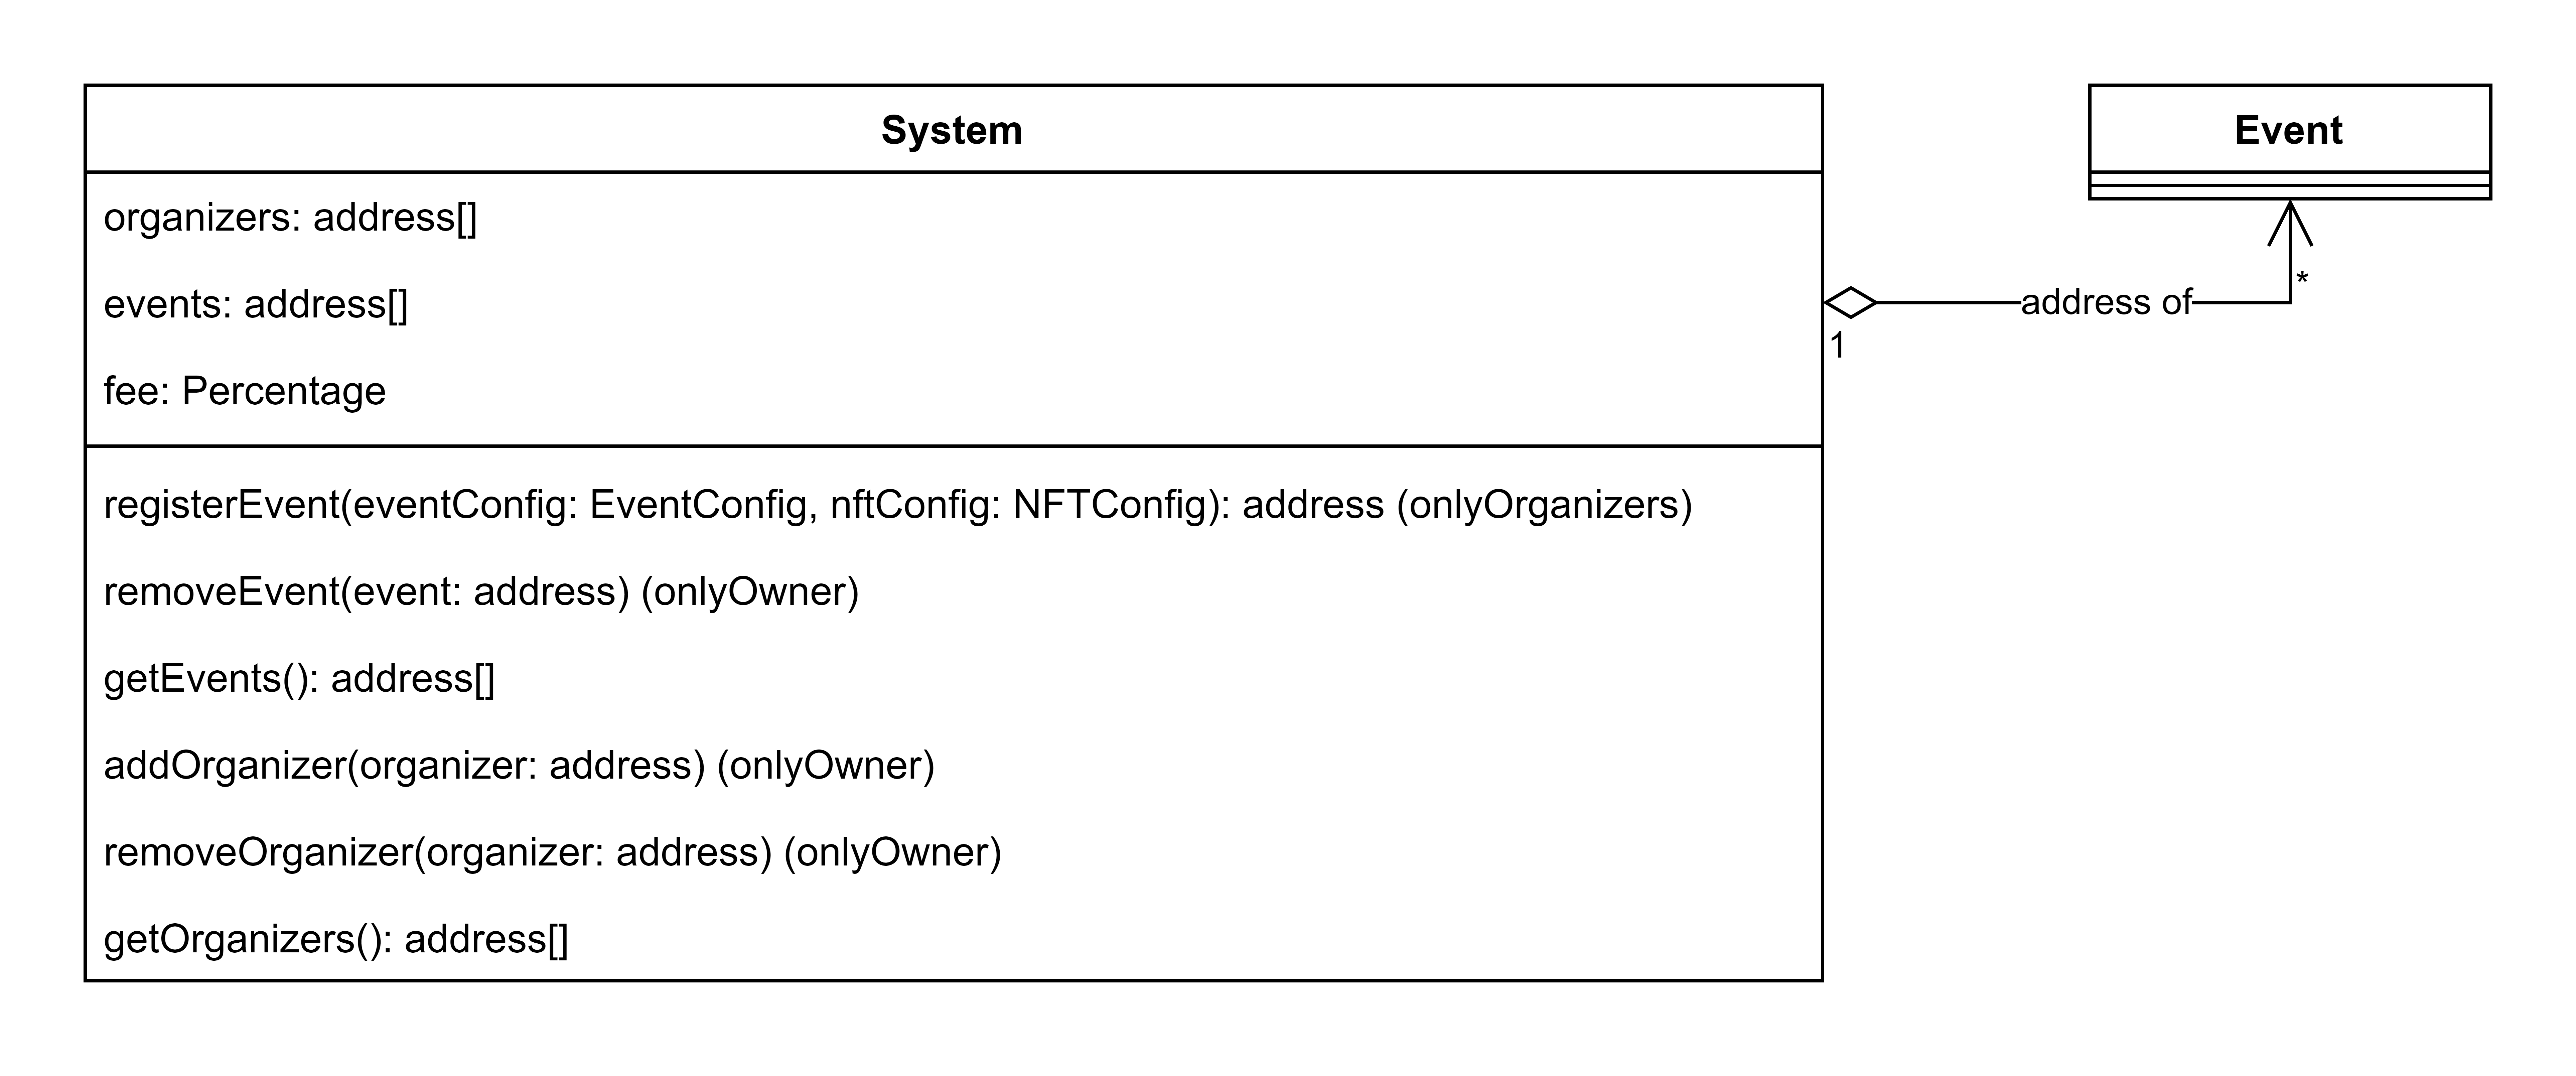
\includegraphics[width=\textwidth]{Main smart contract.png}
    \centering
    \caption{Main smart contract UML}
    \label{fig:main_smart_contract}
\end{figure}


\subsection{Event Smart Contract}
\label{subsec:event_smart_contract}


[erc721]

[structs]

[event smart contract]
- [creation of events]
-- [ipfs (pinata)]
- [structs]
- [event lifecycle]
- [restrictions on ticket operations]

[ticket validation]
[todo mention network fees and network choice]

[user app]
[validator app]

\section{Project Features}
